% ========================================= TEMPLATE INFO ========================================
%
% Author:       P4ntomime
% Version:      1.0.0
% Last updated: 2024-02-18
% Brief:        A LaTeX template for summaries. See README.md for more information.
% 
% ================================================================================================
\documentclass[8pt, a4paper, twoside]{extarticle}
% Font size:    8pt
% Paper size:   A4
% style:        twoside (needed, so odd and even pages have different margins)
% orientation:  portrait. (use 'landscape' for landscape orientation)


% ========================================= DOCUMENT INFO =========================================
\def\title{Analog Microelectronics}                             % title
\def\shorttitle{AnME}                                           % short title (displayed as PDF title)
\def\dozent{Prof. Dr. Paul Zbinden}                             % lecturer
\def\semester{HS 2024}                                          % semester
\def\author{Flurin Brechbühler, Laurin Heitzer, Simone Stitz}   % authors
\def\repo{https://github.com/flurin-b/AnME}                     % repository link
\def\version{1.0.\today}                                        % version
\def\pagelimit{20}                                              % page limit -> causes pages after limit to be red
\def\titleoption{ultra compact}                                 % options: compact, normal
\def\enableToC{true}                                            

% ================================= PACKAGES, SETUP AND COMMANDS ==================================
\input{preamble.tex}

\newcommand{\mytext}[1]{\quad\text{#1}\quad}

% =========================================== DOCUMENT ============================================
\begin{document}
    \begin{layout}
        \part{AnME}
        % CHECK: Lernziele
% • Sie können mindestens zwei Bereiche nennen, in
% denen Analogschaltungen heute in integrierten
% Schaltungen zur Anwendung kommen.
% • Sie kennen die Hauptschritte der Herstellung von
% integrierten Schaltungen in CMOS-Technologie.
% • Sie können die wichtigsten aktiven und passiven
% Bauelemente nennen und beschreiben, die in einem
% CMOS-Prozess standardmässig zur Verfügung
% stehen.

\section{CMOS Technologie}

% NOTE: outcommented due to space issues
% \subsection{Geschichte} 
% \begin{description}
%     \item[1926] Julius E. Lilienfeld: Erster Vorschlag zur Realisierung eines SperrschichtFET
    
%     \item[1934] Oskar Heil: Erster Vorschlag eines Feldeffektverstärkers (Vorläufer vom MOSFET)
%     \item[1947] W. H. Brattain, J. Bardeen (und William B.Shockley): Erfindung des ersten Bipolartransistors
%     \item[1958] Jack S. Kilby: Erste Gedanken zur Realisierung einer integrierten Schaltung
%     \item[1961] Robert W. Noyce: Erhält Patent für die integrierte Schaltung
%     \item[1947] W. Shockley, J. Bardeen und W. Brattain: Erster funktionierender Bipolartransistor \rightarrow Physik-Nobellpreis
%     \item[1958] Jack S. Kilby: Erstes IC mit 1 Transistor, \qty{17.76}{\square\milli\meter}, Realisiert RC-Oszillator
%     \item[2024] Intel: Arrow Lake, >123\,Mio.Tr./mm$^2$
%     \item[2024] Apple: M4max, >92\,Mio.Tr./mm$^2$
% \end{description}

% \paragraph{Moores Law}
% 1965 hat G.E. Moore in einem Paper prognostiziert, dass sich die Transistorzahl pro chip in nächsten 10 Jahren jährlich verdoppeln wird. 
% 1975 wurde die Prognose revidiert auf eine Verdoppelung alle zwei Jahre.


\subsection{Prozessüberblick -- Herstellung integrierter Schaltungen}
Die Herstellung integrierter Schaltungen zeichnet sich durch folgende Besonderheiten aus:
\begin{itemize}
    \item Komplexe Logistik aufgrund einer Vielzahl an Prozessschritten
    \item Hochgradige Standardisierung
    \item Teure Infrastruktur und teure Prozesse
\end{itemize}

\smallskip

Der Prozess läuft in groben Zügen wie folgt ab:
\begin{enumerate}
    \item Sand wird geschmolzen und gereinigt. Daraus wird ein Silizium-Einkristall gezogen.
    \item Der Einkristall wird in Wafer geschnitten / gesägt.
    \item Durch wiederholte Oberflächenbeschichtung, Fotolithografie, Ätzen und Dotierung wird der Wafer strukturiert. Dazwischen muss der Wafer jeweils gesäubert werden.
    \item Die einzelnen Chips auf dem Wafer werden vereinzelt.
    \item Zur Konfektion werden die Chips in Gehäuse verbaut.
    \item Um die ICs in Systemen einzusetzen, werden diese auf Leiterplatten verbaut.
\end{enumerate}

\medskip

% TODO: [Flurin] I hate this image. I'll see if i get round to find a better one.

\begin{minipage}[t]{0.5\columnwidth}
    \includegraphics[width=\columnwidth, align=t]{images/technologie_grundprozess_skript.pdf}
\end{minipage}
\hfill
\begin{minipage}[t]{0.48\columnwidth}
    \paragraph{Lithographie}
    Lichtempfindlicher Lack (Photoresist) wird durch eine Lichtquelle löslich (positiver Photoresist) oder unlöslich (negativer Photoresist) gemacht.
    Durch Lösen des löslichen Photoresists kann die Oberfläche lokal geschützt werden und so gezielt regionen des Chips geätzt oder beschichtet werden.
    Zum Ende wird der übrige Lack entfernt und der Vorgang beliebig oft wiederholt.
\end{minipage}


% \paragraph{Lithographie}
% Das Prinzip der Lithographie basiert auf einem lichtempfindlichen Lack, dem sogenannten Photoresist.
% Dieser wird durch eine Lichtquelle löslich (positiver Photoresist) oder unlöslich (negativer Photoresist) gemacht.
% Durch lösen des löslichen Photoresists kann die Oberfläche lokal geschützt werden und so gezielt regionen des Chips geätzt oder beschichtet werden.
% Zum Ende wird der übrige Lack entfernt und der Vorgang beliebig oft wiederholt.


\paragraph{Ätzen}
Durch Ätzen kann gezielt Material von freiliegenden Flächen des Wafers entfernt werden.
Dabei werden folgende Verfahren unterschieden:
\begin{description}
    \item[Isotrop (Nass oder Plasma):] Gleichförmiges Ätzen in alle Richtungen \rightarrow Bringt die Gefahr des Unterätzens
    \item[Anisotrop (Reactive Ion Etching, KOH oder Plasma):] Ätzen entlang Kristallrichtungen, z.B. KOH greift die (111)-Ebene kaum an \rightarrow Ermöglicht steiliere Gräben, MEMS
    \item[Selektiv:] Selektives Ätzen bestimmter Materialien, z.B. HF ätzt SiO$_2$ aber nicht Si \\
        \rightarrow Erlaubt das Ätzen einer Lage ohne beschädigung unterliegender Strukturen
\end{description}

\paragraph{Dotieren}
Beim Dotieren werden gezielt Fremdatome in den Siliziumkristall eingebracht.
\begin{description}
    \item[Donatoren,] also Atome mit einem Valenzelektron mehr als der Halbleiter, verursachen einen Elektronenüberschuss, der Kristall wird \textbf{n-dotiert}.
    \item[Akzeptoren,] also Atome mit einem Valenzelektron weniger als der Halbleiter, verursachen einen Lochüberschuss, der Kristall wird \textbf{p-dotiert}.
\end{description}


\subsubsection{Backend Prozesse}

\paragraph{Wafer Sort}
Die Chips werden auf dem Wafer einzeln getestet (Kontaktierung mit Nadeln). 
Dies ist oft zeitaufwendig \rightarrow Durch gutes Design sollte diese Zeit minimiert werden.

Der Yield, (prozentualer Anteil funktionaler Chips) hängt dabei von der Chipgrösse ab.
Dies, da jeder Defekt bei grossen Chips eine grosse Fläche beeinträchtigt, da jeweils nur ganze Chips funktionsfähig oder defekt sein können.

Yields von \qty{90}{\percent} sind meist notwendig, um Profit zu machen.

\paragraph{Assembly and Test}
Die Wafer werden in einzelne Chips getrennt und die funktionierenden Chips in Gehäuse verbaut. Im Gehäuse erfolgt ein Final-Test.


\subsection{Arten von Toleranzen}
Bei der Herstellung von Wafern werden verschiedene Toleranzen unterschieden:
\begin{description}
    \item[Devicetoleranz] Toleranzen betreffend der Strukturen auf gleichem Chip
    \item[Prozesstoleranzen] Toleranzen betreffend der Strukturen auf einem Wafer
    \item[Lostoleranz] Toleranzen innerhalb eines Batches bzw. Los (meist 25, selten bis 50 Wafer)
\end{description}

\subsection{CMOS Bauelemente}
Mögliche Strukturen und Elemente wie auch die Materialeigenschaften werden im \textbf{Technologiehandbuch} gegeben.

% NOTE: svg code:
% \subsubsection{NMOS und PMOS Transistoren}
% \begin{center}
%     \includesvg[scale=0.3]{images/01_CMOS.svg}
% \end{center}

% \subsubsection{Bipolartransistoren}
% \begin{center}
%     \includesvg[scale=0.3]{images/01_BJT.svg}
% \end{center}

\subsection{Bipolartransistoren}
\begin{center}
    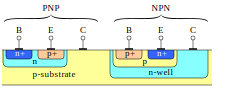
\includegraphics[width=0.5\columnwidth, align=t]{images/01_BJT.pdf}
\end{center}

\subsubsection{Kapazitäten (pro Fläche)}

\vspace{-0.3cm}

$$ \boxed{ C = \varepsilon \cdot  \frac{A}{d} = \varepsilon_0 \cdot \varepsilon_r \cdot \frac{W \cdot L}{d} =  C'' \cdot A } \qquad \qquad
    \boxed{ C'' = \frac{\varepsilon}{d} = \frac{\varepsilon_0 \cdot \varepsilon_r}{d} } $$

\begin{minipage}[t]{0.44\columnwidth}
    \begin{tabular}{l@{}}
        $\varepsilon_0 = \qty{8.85e-12}{\farad\per\meter}$                      \\
        $\varepsilon_{r, \text{Si, SiO$_2$}} \approx 3.9$                       \\
        $\varepsilon_{r, \text{Dielektrikum}} \approx 2.9$ (möglichst klein)   
    \end{tabular}   
\end{minipage}
\hfill
\begin{minipage}[t]{0.55\columnwidth}
    \begin{tabular}{lll@{}}
        $C''$   & Spezifische Kapazität & $[C''] = \qty{}{\farad\per\square\meter}$ \\
        $A$     & Fläche der Kapazität  & $[A] = \qty{}{\square\meter}$             \\
        $d$     & Abstand (fix)         & $[d] = \qty{}{\meter}$
    \end{tabular}
\end{minipage}


% \[
%     \epsilon_0 = \qty{8.85e-12}{\farad\per\meter}
% \]
% \[
%     \epsilon_{r, \text{Si, SiO$_2$}} \approx 3.9
% \]
% \[
%     \epsilon_{r, \text{Dielektrikum}} \approx 2.9 \text{\ (Typisch, so klein wie möglich)}
% \]
% \[
%     C''\text{: Spezifische Kapazität}
% \]

\paragraph{MIM}
Metal-Interconnect-Metal-Kondensatoren produzieren \textbf{sehr kleine Kapazitäten}, da die Interconnect-Layers relativ dick sind ($d \sim \qty{2.5e-7}{\meter}$) und absichtlich aus 'schlechtem' Dielektrikum ($\varepsilon_r \approx 2.9$) bestehen.
Die Spannungsfestigkeit ist jedoch höher.

\paragraph{MOS}
Da Oxidschichten sehr dünn realisiert werden können ($d \sim \qty{2.33e-9}{\meter}$) und ein höheres $\varepsilon_r \approx 3.9$ besitzen, benötigen MOS-Kondensatoren im Vergleich zu MIM-Kondensatoren bedeutend weniger Fläche.
Somit können grössere Kapazitäts-Werte realisiert werden.
Sie besitzen jedoch eine kleinere Spannungsfestigkeit.


\subsubsection{Spulen}
Spulen sind nur planar möglich und beanspruchen oft viel Platz.

\subsubsection{Widerstände (pro quadr. Flächeneinheit)}

\begin{minipage}[c]{0.48\columnwidth}
    $$ \boxed{ R = \rho \frac{L}{A} = \rho \frac{L}{t \cdot W} = R_\square \frac{L}{W} = R_\square \cdot n_\square } $$
    $$ \boxed{ R_\square = \frac{\rho}{t} } $$
\end{minipage}
\hfill
\begin{minipage}[c]{0.5\columnwidth}
    \paragraph{Typische Werte}

    \begin{tabular}{@{}l l@{}}
        Metall              & $R_\square \approx 0.02 ... \qty{0.08}{\ohm}$                  \\
        Poly (salicide)     & $R_\square \approx \qty{10}{\ohm}$                             \\
        Poly (non-salicide) & $R_\square \approx \qty{100}{\ohm}$ (n+ Poly)                  \\
                            & $R_\square \approx \qty{400}{\ohm}$ (p+ Poly)                  \\
        n- / p-Diffusion    & $R_\square \approx 100/\qty{150}{\ohm}$                        \\
        n- / p-Well         & $R_\square \approx 400/\qty{1600}{\ohm}$                       \\
    \end{tabular}
\end{minipage}


% \begin{center}
%     \boxed{
%         R = \rho \frac{L}{A} = \rho \frac{L}{t \cdot W} = R_\square \frac{L}{W}
%     }
% \end{center}
% \begin{center}
%     \boxed{
%         R_\square = \frac{\rho}{t}
%     }
% \end{center}


\subsubsection{Parasitäre Effekte}

Jedes Bauteil ist von parasitären Effekten betroffen. 
Diese sind:
\begin{itemize}
    \item Streukapazitäten und ungewollte Kapazitäten zu anderen Layern
    \item Wiederstandsbelag des Leitermaterials
    \item Induktivitätsbelag von 'langen' Leitern
    \item Toleranzen
    \item Nichtlinearitäten z.B. die Spannungsabhängigkeit der Kapazitäten von PN-Übergängen
\end{itemize}

\smallskip

\textbf{\rightarrow Empfehlung: Verhältnisse verwenden, nicht Absolutwerte!}


        \section{MOS Transistoren}

\subsection{Dotierung}
\begin{center}
    \begin{tabular}{lll}
        \textbf{Dotierung:}          & N-dotiert            & P-dotiert \\
        \textbf{Unreinheit:}         & Aluminium (HG III)   & Phosphor / Arsen (HG V) \\
        \textbf{Majoritätsträger:}   & Elektronen           & Löcher \\
        \textbf{Minoritätsträger:}   & Löcher               & Elektronen \\
    \end{tabular}
\end{center}


\subsection{MOS-Kapazität}
\begin{minipage}[t]{0.5\columnwidth}
    Minoritätsträger werden an das Gate gezogen.
    Die entstandene Raumladungszone weist bei ausreichend hoher Gate-Spannung einen Minoritätsträgerüberschuss auf, ist also in der Funktion \textbf{komplementär} zum Substrat dotiert.
\end{minipage}
\hfill
\begin{minipage}[t]{0.48\columnwidth}
    \includegraphics[width=\columnwidth, align=t]{images/02_MOS_kapazitaet.pdf}
\end{minipage}


\subsection{MOS-Transistoren}
Werden links und rechts vom MOS-Kondensator komplementär zum Substrat dotierte Regionen (Drain und Source) erstellt, so kann ohne Gatespannung aufgrund der PN-Übergänge kein Strom vom Drain zur Source (oder umgekehrt) fliessen.
Wird nun eine Spannung am Gate angelegt, so entsteht die Minoritätsträger-Leitende Raumladungszone - der Kanal.
Dieser verbindet Drain und Source, es kann also ein Strom fliessen.

\vspace{-0.2cm}

\begin{center}
    \includegraphics[width=0.5\columnwidth, align=t]{images/02_CMOS.pdf}
\end{center}


\subsubsection{Übersicht und Symbole}

\begin{minipage}[t]{0.48\columnwidth}
    Durch Vordotierung des Kanals kann der Transistor ohne Gate-Spannung leitend gemacht werden (Verarmungstyp, selbstleitend).
    Eine negative Gate-Spannung kann den Kanal dann abschnüren. \\
    \rightarrow\ hier nicht weiter behandelt

    \smallskip

    \textbf{Der Bulk wird nur eingezeichnet, wenn dieser \myul{nicht} mit $\bm{V_{\rm DD}}$ bzw. $\bm{V_{\rm SS}}$ verbunden ist.}
    Deshalb werden meist die vereinfachten Symbole verwendet:

    \vspace{-0.3cm}

    \begin{center}
        \includegraphics[width=0.8\columnwidth, align=t]{images/02_MOSFET_symbole_vereinfacht.pdf}
    \end{center}
\end{minipage}
\hfill
\begin{minipage}[t]{0.5\columnwidth}
    \includegraphics[width=\columnwidth, align=t]{images/02_MOSFET_uebersicht.pdf}
\end{minipage}



\subsubsection{Modelle}
In Cadence sind verschiedene Modelle hinterlegt:

\textbf{Spice Modell 11:} Das Modell 11 beinhaltet ca. 100 Parameter und ist entsprechend genau.

\textbf{Spice Modell 1:} Vergleichbar mit dem Handrechenmodell, welches zwar weniger genau, dafür aber viel einfacher ist. Dennoch beinhaltet es bereits 40 Parameter.

\subsection{Ausgangskennlinie -- Arbeitsbereiche}
 
Die Ausgangskennlinie beschreibt den Zusammenhang $I_D = f(V_{DS}) \big|_{V_{GS} = \text{konst}}$

\begin{minipage}[t]{0.5\columnwidth}
    \includegraphics[width=\columnwidth, align=t]{images/02_MOSFET_ausgangskennlinien.pdf}
\end{minipage}
\hfill
\begin{minipage}[t]{0.48\columnwidth}
    Zwei Arbeitsbereiche: 

    \begin{outline}
        \1 ungesättig (gesteuerter Widerstand)
        \1 gesättigt (Stromquelle)
    \end{outline}

    \medskip

    Die Sättigungsgrenze $V_{\rm DS, sat}$ ist abhängig vom \textbf{Kanalzustand}:

    \begin{outline}
        \1 \textbf{weak inversion:} \\
            $V_{\rm DS, sat} = V_{\rm eff} \approx 5 \cdot V_{\rm temp} \approx \qty{130}{\milli \volt}$ 
        \1 \textbf{strong inversion:} \\
            $V_{\rm DS, sat} = V_{\rm eff} = V_{GS} - V_T$ 
    \end{outline}
\end{minipage}



\subsection{Transferkennlinie -- Ausgangsstrombereiche}


\begin{minipage}[t]{0.55\columnwidth}
    \includegraphics[width=\columnwidth, align=t]{images/02_MOSFET_transferkennlinie.pdf}
\end{minipage}
\hfill
\begin{minipage}[t]{0.42\columnwidth}
    Die Transferkennlinie beschreibt den Zusammenhang $I_D = f(V_{GS})$ 

    \smallskip

    Dabei werden \textbf{5 Ausgangsstombereiche} unterschieden. Diese hängen mit dem \textbf{Kanalzustand} zusammen.

    \smallskip

    Des Weiteren gibt es die Bereiche:

    \begin{outline}
        \1 Sub Threshold: $V_{GS} < V_T$
        \1 Above Threshold: $V_{GS} > V_T$
    \end{outline}
\end{minipage}


\para{Ausgangsstrombereiche}

\scalebox{0.8}{
\begin{tabular}{|l|l|l|}
    \hline
    \textbf{Bereich}                    & \textbf{Mathem. Charakterisierung}            & \textbf{Zugrundeliegender phys. Effekt}                       \\  
    \hline
    \rowcolor[HTML]{F4CCCC} 
    LECK                                & $I_D$ erreicht Minimalwert, der nicht         & Drain- und Source-Substratdiode haben                         \\
    \rowcolor[HTML]{F4CCCC} 
                                        & weiter unterschritten werden kann             & Leckströme ins Subsstrat                                      \\
    \hline
    \rowcolor[HTML]{FFE5BB} 
    EXP                                 & $I_D$ steigt exponentiell mit $V_{GS}$        & Kanal zeigt \textbf{weak inversion}                           \\
    \hline
    \rowcolor[HTML]{FFF2CC} 
    MOD                                 & Keine 'handliche' Formel für $I_D$            & Kanal zeigt \textbf{moderate inversion}                       \\
    \hline
    \rowcolor[HTML]{D9EAD3} 
    QUAD                                & $I_D$ steigt quadratisch mit $V_{GS}$         & Kanal zeigt \textbf{strong inversion}                         \\
    \hline
    \rowcolor[HTML]{CFE2F3} 
    LIN                                 & $I_D$ steigt annähernd linear mit $V_{GS}$    & Geschwindigkeitssättigung der Ladungsträger im Kanal          \\
    \rowcolor[HTML]{CFE2F3} 
                                        & (halb QUAD, halb LIN)                         & im Kanal (nicht weiter beschleunigbar)                        \\
    \hline
\end{tabular}
}

\smallskip

\textbf{Hinweis:} Die Inversion des Kanals beschreibt, wie sehr sich die Polarität geändert ('invertiert') hat. 
Bei einem n-Kanal FET ist der Kanal ursprünglich p-leidend.
Wird der Kanal invertiert, so wird er (schwach, moderat oder start) n-leitend. 


\subsection{Ersatzschaltungen}

Je nach Arbeitsbereich (gesättigt / ungesättigt) müssen verschiedene Ersatzschaltungen verwendet werden.

\begin{minipage}[t]{0.48\columnwidth}
    \raggedright

    \subsubsection*{Ungesättigt}

    Gesteuerter Widerstand \rightarrow\ $I_D = f(V_{DS})$
    
    \includegraphics[width=\columnwidth, align=t]{images/02_MOSFET_ersatzschaltung_ungesaettigt.pdf}

    \smallskip
    Je kleiner $r_{\rm DS0}$, desto steiler die Geraden links im Ausgangskennlinienfeld

\end{minipage}
\hfill
\begin{minipage}[t]{0.48\columnwidth}
    \raggedright

    \subsubsection*{Gesättigt}

    Stromquelle \rightarrow\ $I_D = f(V_{GS})$

    \includegraphics[width=\columnwidth, align=t]{images/02_MOSFET_ersatzschaltung_gesaettigt.pdf}

    \smallskip
    Je grösser $r_{\rm DS}$, desto flacher die Geraden rechts im Ausgangskennlinienfeld
\end{minipage}


\subsection{Berechnung des Drainstroms}

% CHECK [Simi] @Flurin (gnaze subsection): Formeln für p-Kanal UND n-Kanal? (im Skript ist beides, in den Slides nicht)
% CHECK [Simi] @Flurin (gnaze subsection): Kanallängenmodulation Faktor $(1 + \lambda)$ bei Formeln hinzufügen? (ist im Skript enthalten, in den Slides nicht)

Die Berechnung des Drainstroms hängt sowohl von Arbeitsbereich (gesättigt / ungesättig), als auch vom Ausgangsstrombereich (bzw. der Kanaliversion) ab!


\subsubsection{Strong Inversion}

\vspace{-0.3cm}

$$ \boxed{ \text{QUAD-Bereich: } V_H(I_D) < V_{GS} < V_L(I_D) } \qquad \qquad \beta = \mu \cdot C_{\text{OX}} \cdot \frac{W}{L} $$


\renewcommand{\arraystretch}{1.5}
\begin{ctabular}{c|c}
    \textbf{Ungesättigt}                                                            & \textbf{Gesättigt}                        \\
    $I_D = \beta \cdot \bigg[ (V_{GS} - V_T) V_{DS} - \frac{V_{DS}^2}{2} \bigg]$    & $I_{\text{D, ideal}} = \frac{\beta}{2} (V_{GS} - V_T)^2$\\
    $I_D = \beta \cdot \bigg[ (V_{GS} - V_T) V_{DS} - \frac{V_{DS}^2}{2} \bigg]$    & $I_{D} = \frac{\beta}{2} (V_{GS} - V_T)^2 \cdot (1 + \lambda \cdot \Delta V_{DS})$
\end{ctabular}
\renewcommand{\arraystretch}{1}

%TODO: V3S9 nochmal studieren, macht iwie noch nicht so sinn.
\paragraph{Kanallängenmodulation $\lambda$}
\[
    \lambda = \frac{1}{V_E} % \overset{V_E >> V_{DS}}{\approx} \frac{1}{V_E}
\]
Die Early-Spannung $V_E = a_E \cdot L$ setzt sich zusammen aus dem technologieabhängigen Early-Faktor $a_E$ und der Kanallänge $L$.
%CHECK: Ich finde die Herleitung aus V3S9 überflüssig. Evtl. macht die Grafik zur Early-Spannung sinn? Braucht halt viel platz...

\paragraph{Body-Effekt}
Der Body-Effekt beschreibt die Abhängigkeit der Schwellenspannung $V_T$ von der Source-Bulk-Spannung als
\[
    V_T = V_{T0} \pm \Delta V_T \quad \text{mit} \quad \gamma\left(\sqrt{\abs{V_{SB}+\abs{2\Phi_F}}}-\sqrt{\abs{}}\right).
\]

Das Fermi-Potential
\[
    \Phi_F = kT/q \ln(N_A/n_i)
\]
mit 
\begin{tabular}{rl}
    $n_i$:& Intrinsische ladungsdichte von Silizium\\
    $N_A$:& Ladungsdichte der Akzeptoren
\end{tabular}
ist Prozess- wie auch Temperaturabhängig.
Zudem ist er abhängig der Dotierungsstärke.



Body-Effekt-Konstante
\[
    \gamma \overset{\approx}{n-Dotierung} \qty{1.46}{\sqrt{\volt}}
\]
\[
    \gamma \overset{\approx}{p-Dotierung} \qty{1.08}{\sqrt{\volt}}
\]
\paragraph{Transkonduktanz-Parameter}
$\beta$ ist abhängig davon, ob der Transistor gesättigt ist. 
In der Praxis wird diese Unterscheidung jedoch nicht gemacht. 
Beta ist jedoch gegeben durch 
\[
    \beta = \beta_0 \frac{W}{L} = \mu C_{OX} \frac{W}{L}
\]
und so abhängig von der Kanalbreite $W$ und -länge $L$.

%TODO: NMOSI und PMOSI V2S12


\subsubsection{Weak Inversion}

\vspace{-0.3cm}

$$ \boxed{ \text{EXP-Bereich: } V_K(I_D) < V_{GS} < V_M(I_D) \qquad \qquad V_M(I_D) = V_T(I_D) - x_M(I_D) } $$

%TODO bzw CHECK [Simi] @Flurin Vtemp Formel auch irgendwo ergänzen? Wert für Vtemp in Übungen immer aus Technologiehandbuch gegeben
% CHECK [Flurin] @Simi Würde ich in die FoSa nemen falls an der Prüfung nicht gegeben. Habe aber noch einen disclaimer eingebaut.
Dabei wird $V_{\rm temp}$ oft vom Technologiehandbuch gegeben. 

Alternativ kann sie als 

\begin{minipage}{0.4\columnwidth}
    \[
        V_{\rm temp} = \frac{kT}{q} \approx \qty{130}{\milli\volt}
    \]
\end{minipage}
\hfill
\begin{minipage}{0.5\columnwidth}
    \begin{tabular}{rl}
        $k$: & Boltzmann-Konstante \\
        $q$: & Elementarladung \\
        $T$: & Temperatur in Kelvin \\
    \end{tabular}
\end{minipage}

% CHECK: Ist das tatsächlich eine approximation? Was stimmt nicht daran?
% CHECK: Wovon kommen die 130 mV? -> Gesehen in Quiz zu Woche 2
approximativ berechnet werden.

\renewcommand{\arraystretch}{1.5}
\begin{ctabular}{c|c}
    \textbf{Ungesättigt}                                                                                                & \textbf{Gesättigt}                                                    \\
    $I_D = I_M \cdot \e^{\frac{V_{GS} - V_M}{n_M \cdot V_\text{temp}}} \cdot (1 - \e^{-\frac{V_{DS}}{V_\text{temp}}})$  & $I_D = I_M \cdot \e^{\frac{V_{GS} - V_M}{n_M \cdot V_\text{temp}}}$
\end{ctabular}
\renewcommand{\arraystretch}{1}

\paragraph{Temparaturspannung}
\[
    V_{temp} = \frac{k T}{q} \approx \qty{86.2}{\micro\volt\per\kelvin} \cdot T
\]

\paragraph{Spezifischer Drainstrom}
\[
    I_M = \frac{W}{L} I_{M, 0}
\]

\paragraph{Subthreshold Slope Factor}
\[
    n_M = 1 + \frac{\gamma}{2\sqrt{V_{SB}+\Phi_0}} \quad \text{mit} \quad \Phi_0 = 2 \Phi_F \approx \qty{0.6}{\volt}
\]

\paragraph{Kanallängenmodulation}
\[
    \lambda = \frac{1}{V_E} \approx \frac{1}{a_E L}
\]

\paragraph{Transkonduktanz-Parameter}
\[
    \beta = \frac{W}{L}\beta_0 = \mu C_{OX}
\]
(unter Vernachlässigung der Abhängigkeit von der Sättigung.)

\subsubsection{Bereiche ohne Berechnungsformeln}

In den drei verbleibenden Bereichen sind \textbf{keine Berechnungsformeln für} $\bm{I_D}$ vorhanden.

\smallskip

\begin{minipage}[c]{0.48\columnwidth}
    \renewcommand{\arraystretch}{1.2}
    \begin{ctabular}{lll}
        \textbf{Bereich}    & \textbf{Grenzen}                  \\
        LECK                & $V_K(I_D) < V_{GS} < V_M(I_D)$    \\ 
        MOD                 & $V_M(I_D) < V_{GS} < V_H(I_D)$    \\ 
                            & $V_H(I_D) = V_T(I_D) + x_H(I_D)$  \\
        LIN                 & $V_L(I_D) < V_{GS}$               \\ 
    \end{ctabular}
\end{minipage}
\hfill
\begin{minipage}[c]{0.48\columnwidth}
    Im MOD-Bereich (moderate inversion) liefern die Formeln der weak bzw. strong inversion katastrophal falsche Resultate!

    \smallskip

    Es ist daher enorm wichtig, den Arbeitsbereich des Transistors korrekt zu bestimmen.
\end{minipage}


\subsection{Modellierung}
\subsubsection{Bestimmung des Arbeitspunkts}
Um den Zustand eines MOS-FET zu bestimmen, wird wie folgt vorgegangen:
\begin{enumerate}
    \item $V_{GS}$ bestimmen
    \item Ausgangsstrombereich (weak, strong inversion, \ldots) anhand von Vergleich von $V_{GS}$ mit $V_K$, $V_M$, $V_T$, $V_H$ und $V_L$
    \item $V_{DS}$ ermitteln
    \item $V_{DS, sat}$ ausrechnen
    \item Ausgangsspannungsbereich durch vergleich von $V_{DS}$ mit $V_{DS, sat}$ ermitteln (gesättigt vs. ungesättigt)
\end{enumerate}

\subsubsection{Modellieren im Arbeitspunkt}
Um eine Transistorschaltung zu erstellen muss wie folgt vorgegangen werden:
\begin{enumerate}
    \item Definieren des Arbeitspunkts
    \item Linearisierung im Arbeitspunkt mittels ersatzschaltung
    \item Mit den linearisierten Grössen rechnen
\end{enumerate}
%TODO: Ergänzte Ersatzschaltung -> Evtl. vorherige entfernen?

\subsubsection{Ersatzschaltbilder}
\paragraph{Grosssignalersatzschaltbild}
Zur Bestimmung des Arbeitspunkts bzw. aller Gleichspannungen.
\begin{description}
    \item[AC-Spannungsquellen] durch Kurzschlüsse ersetzen.
    \item[AC-Stromquellen] durch Unterbrüche ersetzen. 
    \item[Kondensatoren] durch Unterbrüche ersetzen.
    \item[Spulen] durch Kurzschlüsse ersetzen.  
\end{description}

\paragraph{Kleinsignalersatzschaltbild}
Zur Berechnung von Verstärkungsfaktoren und Eingangswiderständen für AC-Signale.
\begin{description}
    \item[DC-Spannungsquellen] durch Kurzschlüsse ersetzen.
    \item[DC-Stromquellen] durch Unterbrüche ersetzen. 
    \item[Nichtlineare Bauteile] durch deren Kleinsignalersatzschaltbild ersetzen.
    \item[Koppel- und Bypass-Kondensatoren] durch Kurzschlüsse ersetzen.  
\end{description}
        \section{MOSFET Grundschaltungen}
Es werden drei Grundschaltungen unterschieden. 
Diese werden jeweils durch deren Common-Anschluss benannt.

\begin{center}
    \begingroup\rowcolors{1}{white}{gray!25}
    \begin{tabular}{|c|ccc|}
        \hline
        Schaltung   & Source-Schaltung & Gate-Schaltung & Drain-Schaltung \\
        \hline
        Common      & Source    & Gate      & Drain     \\
        Eingang     & Gate      & Source    & Gate      \\
        Ausgang     & Drain     & Drain     & Source    \\
        \hline
    \end{tabular}\endgroup
\end{center}


\subsection{Einsatzgebiete und Eigenschaften}

\begin{center}
    \begingroup\rowcolors{1}{white}{gray!25}
    \begin{tabular}{|cccc|}
        \hline
        Grundschaltung          & Anwendung & $r_{in}$ & $r_{out}$ \\
        \hline
        Source                  & Tiefe -- mittlere Freq. & gross & gross \\
        Gate                    & Hohe Freq. & klein & gross \\
        Drain / Source-Folger   & Spannungsfolger, Treiber & gross & klein \\
        \hline
    \end{tabular}\endgroup
\end{center}

\subsection{Dimensionieren}
\begin{easylist}
    \ListProperties(Style1*=\bfseries,Numbers2=l,Mark1={},Mark2={)},Indent2=1em)
    @ Arbeitspunkt bestimmen
    @ Kleinsignalersatzschaltung
    @@ Beschaltung umzeichnen
    @@ Transistor durch Ersatzschaltbild ersetzen
    @ Durch lineare Analyse $a$ und $r$ berechnen
\end{easylist}

\subsection{Source-Schaltung}
% TODO: Source-Schaltung aus (oder wie in) V5S6

\subsubsection{Verstärkung}
\[
    a = \frac{v_{out}}{v_{in}} = \frac{R_D}{R_S + \frac{1}{g_m} + \frac{g_0}{g_m}(R_D + R_S)} \overset{R_G = R_S = 0}{=} - g_m (r_{ds} || R_D)
\]

\paragraph{Optimierung}
\begin{itemize}
    \item $R_S$ und $R_D$ weglassen um Chipplatz zu sparen.
    \item $R_D \to \infty$ (so gross wie möglich)
\end{itemize}

\textbf{Strong Inversion}
\[
    r_{DS} = \frac{a_E \cdot L}{I_D} \qquad g_m = \mu C_{OX} \frac{W}{L} (V_{GS} - V_T) = \frac{2 I_D}{V_{GS}-V_T}
\]
\[
    a_{max} = - \frac{g_m}{g_0} = -g_m r_{DS} = -\frac{2\cdot a_E \cdot L}{V_{GS} - V_T}
\]
\begin{itemize}
    \item $V_{GS}$ so tief wie möglich wählen ($V_{GS}-V_T \approx 150 - \qty{200}{\milli\volt}$).
    \item $L$ möglichst gross wählen.
\end{itemize}

\textbf{Weak Inversion}
\[
    g_{m} = \frac{I_D}{n_m V_{temp}} \qquad r_{DS} \approx \frac{a_E \cdot L}{I_D}
\]
\[
    a_{max} = - \frac{g_m}{g_0} = -g_m r_{DS} = -\frac{\cdot a_E \cdot L}{n_m - V_{temp}}
\]
\begin{itemize}
    \item In Weak Inversion erreicht der Transistor seine maximale Verstärkung.
    \item Sie wird durch Technologieparameter sowie $L$ bestimmt.
    \item Da mit in Weak Inversion mit Nähreungsformeln gerechnet wird, muss simuliert werden.
\end{itemize}

\subsubsection{Notizen}
\begin{itemize}
    \item Invertiert das Eingangssignal.
    \item $a_{max}$ ist der Grenzwert der Verstärkung, nicht die tatsächliche Verstärkung!
\end{itemize}

\subsection{Gate-Schaltung}
% TODO: Gate-Schaltung aus (oder wie in) V5S6

\subsubsection{Verstärkung}
\[
    a = \frac{v_{out}}{v_{in}} = \frac{R_D (1+\frac{g_0}{g_m})}{R_S + \frac{1}{g_m} + \frac{g_0}{g_m} (R_D + R_S)}
\]

\paragraph{Optimierung}
\textbf{Strong Inversion}
Für $R_S = 0$ und $R_D << 1/g_0$ gilt
\[
    a \overset{R_D \text{klein}}{\approx} g_m R_D \quad \text{bzw.} \quad a \overset{R_D \text{gross}}{\approx} \frac{g_m}{g_0} = a_{max}.
\]

%TODO: Weak inversion Grenzwerte? Oder einfach Verweis auf Source-Schaltung?

\subsubsection{Notizen}
\begin{itemize}
    \item Ohne Body-Effekt erreicht die Gate-Schaltung die gleiche Verstärkung wie die Source-Schaltung mit besserem Frequenzverhalten.
    \item Bei der Gate-Schaltung wird der Body-Effekt schnell zum Problem.
\end{itemize}

\subsection{Drain-Schaltung (Source-Follower)}
% TODO: Drain-Schaltung aus (oder wie in) V5S6

\subsubsection{Verstärkung}
\[
    a = \frac{v_{out}}{v_{in}} = \frac{R_S}{R_S + \frac{1}{g_m} + \frac{g_0}{g_m} (R_D + R_S)}
\]

\paragraph{Optimierung}
\[
    a_{max} = \lim_{R_S \to \infty} a \overset{g_m >> g_0 und r_{DS} >> R_D}{=} \lim_{R_S \to \infty} g_m \frac{R_S}{g_m R_S + 1} = 1
\]

\paragraph{Level-Shift}
Die Drain-Schaltung reduziert den DC-Pegel des Ausgangssignals um 
\[
    V_{GS} = V_T + \sqrt{\frac{2 I_D}{\mu C_{OX} \frac{W}{L}}}.
\]

\paragraph{Body Effekt}
Da die Source nicht auf Body-Potential ist, muss die Veränderung der Threshold Spannung $V_T$ aufgrund des Body-Effekts berücksichtigt werden.

\subsubsection{Notizen}
\begin{itemize}
    \item Der Source-Follower hat immer eine Verstärkung $a \leq 1$
    \item Der Source-Follower bewirkt immer einen Level-Shift um $V_{GS}$.
\end{itemize}

\subsection{Eingangs- und Ausgangswiderstände}
\begin{itemize}
    \item Fiktive Spannungsquelle ans Kleinsignalersatzschaltbild anschliessen.
    \item Strom, der über den Sorce-Knoten in den Transistor fliesst, messen.
    \item Widerstand als $r_i = \frac{u_i}{i_i}$ berechnen.
\end{itemize}

\paragraph{am Gate}
\[
    r_{i, G} \to\ \infty
\]
\paragraph{am Drain}
\[
    r_{i, S} = \frac{1}{g_m + g_0} (1 + g_0 R_D)
\]
\[
    r_{i, S} \overset{r_{DS}>>R_D}{\approx} \frac{1}{g_m + g_0}
\]
\[
    r_{i, S} \overset{g_m>>g_0}{\approx} \frac{1}{g_m}
\]
\paragraph{an Der Source}
\[
    r_{i, D} = r_{DS} (1+g_m R_S) + R_S
\]
\[
    r_{i, D} \overset{r_{DS}>>R_S}{\approx} r_{DS} (1+g_m R_S)
\]
\[
    r_{i, D} \overset{R_S = 0}{\approx} r_{DS}
\]
        \section{MOS Diode}
\subsection{Gegenüberstellung Diodentypen}

%NOTE: Platzhalter! -> wird mit überarbeitetem pdf ersetzt
%TODO: [Simi]: pdf
\includegraphics[width=\columnwidth, align=t]{images/04_Vergleich_Dioden.png}


\subsection{Arbeitsbereich der MOS Diode}

Die MOS Diode arbeitet \textbf{(in strong inversion) immer in Sättigung}, da die Sättigungsbedingung aufgrund der Verbindung der Gate- und Source-Anschlüsse immer erfüllt ist:
\[
    V_\text{DS} = V_\text{GS} > V_\text{GS} - V_\text{T}
\]
\textbf{Hinweis:} Die Forwardspannung bestimmt, ob die MOS Diode in strong- oder weak inversion betrieben wird.
\textbf{Der 'Normalfall' ist strong inversion.}


\subsection{Arbeitspunkteinstellung}

\subsubsection{Arbeitspunkteinstellung mittels Drainstrom}

\begin{minipage}[t]{0.3\columnwidth}
    \includegraphics[width=\columnwidth, align=t]{images/04_MOS_diode_mit_stromquelle.pdf}
\end{minipage}
\hfill
\begin{minipage}[t]{0.66\columnwidth}
    Aus der Drainstrom-Gleichung (strong inversion, Sättigung) lässt sich die Spannung über der Diode als Funktion des Eingangsstroms berechnen:
    \[
        V_\text{DS} = V_\text{GS} = V_T + \sqrt{\frac{2 I_\text{D}}{\mu C_\text{ox} \frac{W}{L}}}
    \]

    %CHECK: [Simi] @ Flurin: WO kommt das her? Ist das relevant?   
    \[
        V_{GS} = V_\text{M} + n_M V_\text{temp} \ln{\frac{I_\text{D}}{I_m' \frac{W}{L}}}
    \]
\end{minipage}


\subsubsection{Arbeitspunkteinstellung mittels Seriewiderstand}

\begin{minipage}[t]{0.3\columnwidth}
    \includegraphics[width=\columnwidth, align=t]{images/04_MOS_diode_mit_widerstand.pdf}
\end{minipage}
\hfill
\begin{minipage}[t]{0.66\columnwidth}
    Der Arbeitspunkt kann auf zwei Arten ermittelt werden:

    \smallskip
    
    \begin{outline}
        \1 Grafisch durch Einzeichnen der Lastgerade des Drainwiderstands $R_1$ in der Kennlinie $I_D = f(V_{\rm GS})$
            \2 Leerlaufspannung: $V_{\rm GS,0} = V_{\rm DD}$
            \2 Kurzschluss-Strom: $I_{D, 0} = \frac{V_{\rm DD}}{R_1}$ \\
            \textrightarrow\ Schnittpunkt entspricht Arbeitspunkt
            \smallskip
        \1 Rechnerisch mittels folgender Formel
        $$ I_D = \frac{V_{\rm DD} - V_{\rm GS}}{R_1} = \frac{\mu C_{\rm OX}}{2} \frac{W}{L} (V_{\rm GS} - V_T)^2 $$
    \end{outline}
\end{minipage}


\subsection{Kleinsignalersatzschaltung}

\begin{minipage}[t]{0.3\columnwidth}
    \includegraphics[width=\columnwidth, align=t]{images/04_MOS_diode_ersatzschaltung_vereinfacht.pdf}
\end{minipage}
\hfill
\begin{minipage}[t]{0.65\columnwidth}
    Die Kleinsignalersatzschaltung kann (leicht angepasst) vom MOS Transistor übernommen werden.
    \begin{align*}
        \text{Allgemein:} \quad             r_\text{\rm MD}  &= \frac{1}{g_m + g_0} = \frac{1}{g_m} \parallel r_{DS} \\
        \text{\textbf{Praxis:}} \quad       r_\text{\rm MD} &\approx \frac{1}{g_m} = \frac{1}{\sqrt{2 \mu C_\text{ox} \frac{W}{L} I_\text{D}}}
    \end{align*}

\end{minipage}


\subsection{Anwendungen}

\subsubsection{Spannungsreferenz}
\label{Spannungsreferenz}

\begin{minipage}[t]{0.44\columnwidth}
    \includegraphics[width=\columnwidth, align=t]{images/04_MOS_diode_spannungsreferenz.pdf}
\end{minipage}
\hfill
\begin{minipage}[t]{0.52\columnwidth}
    \textbf{Voraussetzung: } Referenzstrom $I_Q$
    \smallskip

    \begin{itemize}
        \item[+] Kleinerer Flächenanspruch als Widerstand
        \item[+] Eingangsspannung wird durch relativ tiefen $\Delta r_{\rm MD}$ geglättet
        \item[-] Genauer als mit Widerstand, jedoch noch immer eher ungenau
        \item[-] $r_{\rm MD}$ kann nur schlecht verändert werden
    \end{itemize}
\end{minipage}


\subsubsection{Spannungsstabilisator}

\begin{minipage}[t]{0.48\columnwidth}
    \begin{outline}
        \1 MOS-Dioden Schaltung aus Abschnitt \ref{Spannungsreferenz} mit Widerstand statt Stromquelle
        \1 AC-Störung wird oberhalb von $R$ eingespeist (gegenüber GND)
    \end{outline}
\end{minipage}
\hfill
\begin{minipage}[t]{0.48\columnwidth}
    \raggedright
    
    \begin{outline}
        \1 Kleinsignalersatzschaltung des beschriebenen Aufbaus:
            \2 Spannungsteiler aus $R$ (gross) und $r_{\rm MD}$ (klein) \\
            \textrightarrow\ AC-Störspannung $v_0$ am Ausgang ($V_{\rm DS} + v_0$) sehr klein
    \end{outline}
\end{minipage}


% CONTINUE HERE


\subsubsection{Spannungsteiler}
% TODO: Entweder entfernen oder schemen aus V6S13 einfügen, sicher korrektes Schema einfügen
a:
 - body-Effekt bei oberem Transistor

b:
 + Da P-Transistoren kein Body-Effekt
 + Matching gut da beides P-Transistoren

c:
 - Matching schlecht, da komplementäre Elemente
 + Kein Body-Effekt

d:
 - viel Fläche
 - schlechte absolute genauigkeit
 + gute relative genauigkeit
        \section{MOS Stromquelle}
Bei der Einstellung des Arbeitspunkts mittels Widerstand resultiert eine quadratische Gleichung für den Strom und so die Ausgangsspannung eines Verstärkers.
Abhilfe kann eine Stromquelle anstelle des Widerstands schaffen.

MOS Transistoren sind bereits spannungsgesteuerte Stromquellen.
Durch einfügen eines $R_S$ kann der Innenwiderstand der Stromquelle \textbf{maximiert} werden. \textrightarrow\ Quelle wird 'idealer'

\subsection{Stromquelle -- Grundschaltungen}

% TODO: [Flurin] @ Simi: Schaltung mit R_S aus V6S18 und evtl. Formeln für R_iD aus V6S17
%CHECK: [Simi] @ Flurin: Falsche Slide für Schaltung im obigen todo..? Habe jetzt mal improvisiert...

\begin{minipage}[t]{0.44\columnwidth}
    \includegraphics[width=0.48\columnwidth, align=t]{images/05_stromquelle_einfach_NMOS.pdf}
    \includegraphics[width=0.48\columnwidth, align=t]{images/05_stromquelle_einfach_PMOS.pdf}
\end{minipage}
\hfill
\begin{minipage}[t]{0.5\columnwidth}
    \paragraph{Ausgangswiderstand}

    \vspace{-0.4cm}
    % \[
    %     r_{\rm iD} = r_{\rm DS} \left( 1 + g_m R_S + \frac{R_S}{r_{\rm DS}} \right) = r_{\rm DS} (1 + g_m R_S) + R_S 
    % \]

    \begin{align*}
         r_{\rm iD} &= r_{\rm DS} \left( 1 + g_m R_S + \frac{R_S}{r_{\rm DS}} \right) \\ 
                    &= r_{\rm DS} (1 + g_m R_S) + R_S
    \end{align*}
            

    \paragraph{Minimale Ausgangsspannung}

    \vspace{-0.2cm}

    \[
        V_{\rm out} = V_O > V_{O , \rm min} = R_S I_D + D_{\rm DS, sat}
    \]
\end{minipage}


\subsection{Kaskoden}
Damit für die Stromquelle kein Widerstand verwendet werden muss, kann ein weiterer Transistor verwendet werden. Diese Schaltung wird Kaskode genannt.

Dabei wird der maximale Ausgangsstrom jedoch leicht reduziert.


\subsubsection{Kaskode -- Grundschaltung}
\label{Kaskode -- Grundschaltung}

\begin{minipage}[t]{0.3\columnwidth}
    \includegraphics[width=\columnwidth, align=t]{images/05_stromquelle_kaskode.pdf}
\end{minipage}
\hfill
\begin{minipage}[t]{0.62\columnwidth}
    \paragraph{Ausgangswiderstand}

    \vspace{-0.2cm}
    \[
        r_{\rm out} = r_{\rm o2} \approx g_{m2} \cdot r_{\rm DS}^2 = a_{\rm max} \cdot r_{\rm DS}
    \]
            

    \paragraph{Minimale Ausgangsspannung}

    \vspace{-0.5cm}
    \[
        V_{O, \rm min} = V_{\rm G2} - V_{\rm GS2} + V_{\rm DS2, sat} =  V_{\rm DS1, sat} + V_{\rm DS2, sat}
    \]


    \paragraph{Strom}

    \vspace{-0.4cm}
    \[
        I_D = \frac{\mu C_{\rm ox}}{2} \left( \frac{W}{L}\right)_{N1} (V_{\rm GS\_N1} - V_T)^2 \cdot \cbl{(1 + \lambda V_{\rm DS\_N1})}
    \]
\end{minipage}


\subsubsection{Geregelte Kaskode}
Um die Kaskodenschaltung weiter zu \textbf{verbessern}, kann die $V_\text{GS}$ Spannung des oberen Transistors auf die Referenzspannung geregelt werden.
Durch das Stabilisieren der Spannung wird der Arbeitspunkt des Transistors stabilisiert (indem $I_D$ konstant ist) und der \textbf{Ausgangswiderstand noch grösser}.

\smallskip

\begin{minipage}[t]{0.55\columnwidth}
    \includegraphics[width=\columnwidth, align=t]{images/05_stromquelle_geregelte_kaskode_opamp.pdf}
\end{minipage}
\hfill
\begin{minipage}[t]{0.42\columnwidth}

    \paragraph{Transkonduktanz}

    \vspace{-0.3cm}
    \[
        g_{m,\rm super} = g_{m1}
    \]            

    \paragraph{Minimale Ausgangsspannung}

    \vspace{-0.2cm}
    \[
        V_{O, \rm min} =  V_{\rm ref} + V_{\rm DS2, sat}
    \]

    \paragraph{Strom}

    \textrightarrow\ Siehe Grundschaltung (\ref{Kaskode -- Grundschaltung})
\end{minipage}


\paragraph{Ausgangswiderstand}

\vspace{-0.3cm}
\[
    r_{\rm out} \approx r_{\rm DS1} \cdot g_{m2} \cdot r_{\rm DS2} \cdot (a + 1) = \frac{1}{g_{o1}} \cdot \frac{g_{m2}}{g_{o2}} \cdot (a + 1)
\]


\subsubsection{Säckinger Kaskode}
Die Säckinger Kaskode ersetzt den komplexen OpAmp mit einem einzelnen Transistor ($\rm N_3$) in \textbf{Source-Schaltung}.

\smallskip

\begin{minipage}[t]{0.55\columnwidth}
    \includegraphics[width=\columnwidth, align=t]{images/05_stromquelle_geregelte_kaskode_FET.pdf}
\end{minipage}
\hfill
\begin{minipage}[t]{0.42\columnwidth}

    \paragraph{Transkonduktanz}

    \vspace{-0.3cm}
    \[
        g_{m,\rm super} = g_{m1}
    \]            

    \paragraph{Minimale Ausgangsspannung}

    \vspace{-0.2cm}
    \[
        V_{O, \rm min} =  V_{\rm GS3} + V_{\rm DS2, sat}
    \]

    \paragraph{Strom}

    \textrightarrow\ Siehe Grundschaltung (\ref{Kaskode -- Grundschaltung})
\end{minipage}


\paragraph{Ausgangswiderstand}

\vspace{-0.3cm}
\[
    r_{\rm out} \approx r_{\rm DS1} \cdot g_{m2} r_{\rm DS2} \cdot g_{m3} r_{\rm DS3} = \frac{1}{g_{o1}} \cdot \frac{g_{m2}}{g_{o2}} \cdot \frac{g_{m3}}{g_{o3}}
\]


    \end{layout}
\end{document}
